\documentclass[tikz]{standalone}
\usepackage{amsmath}
\usetikzlibrary{arrows.meta}
\definecolor{bg}{HTML}{171D2B}
\definecolor{acc}{HTML}{F7B538}
\begin{document}
\pagecolor{bg}
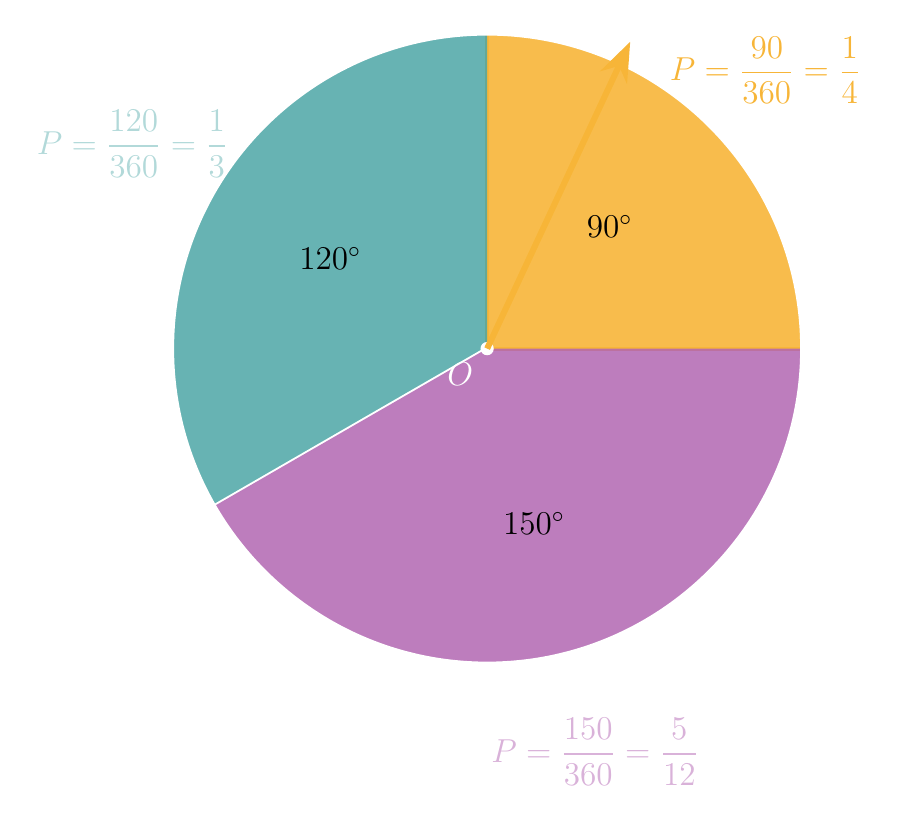
\begin{tikzpicture}[line width=1.4pt,text=white,font=\large]
  % Tiga sektor: 90 (0--90), 120 (90--210), 150 (210--360)
  \coordinate (O) at (0,0);
  \coordinate (A) at (4,0);      % 0 derajat
  \coordinate (B) at (90:4);     % 90 derajat
  \coordinate (C) at (210:4);    % 210 derajat
  % Sektor 1: 90 derajat -> peluang 90/360 = 1/4 (kuning)
  \fill[acc,opacity=0.9] (O) -- (A) arc (0:90:4) -- cycle;
  \draw[acc] (O) -- (A);
  \draw[acc] (O) -- (B);
  % Sektor 2: 120 derajat -> peluang 120/360 = 1/3 (hijau teal)
  \fill[teal!70!white,opacity=0.85] (O) -- (B) arc (90:210:4) -- cycle;
  \draw[white] (O) -- (C);
  % Sektor 3: 150 derajat -> peluang 150/360 = 5/12 (ungu muda)
  \fill[violet!60!white,opacity=0.85] (O) -- (C) arc (210:360:4) -- cycle;
  % Lingkaran utama
  \draw[white] (O) circle (4);
  % Titik pusat dan jarum penunjuk
  \fill[white] (O) circle (2.4pt);
  \node[below left=1pt] at (O) {$O$};
  \draw[-{Stealth[length=5mm]},acc,line width=2.2pt] (O) -- (65:4.3);
  % Label sudut tiap sektor (di tengah sektor)
  \node[black] at (45:2.2) {\textbf{$90^\circ$}};
  \node[black] at (150:2.3) {\textbf{$120^\circ$}};
  \node[black] at (285:2.3) {\textbf{$150^\circ$}};
  % Label peluang di luar lingkaran, searah tengah sektor
  \node[acc] at (45:5.0) {$P=\dfrac{90}{360}=\dfrac14$};
  \node[teal!30!white] at (150:5.2) {$P=\dfrac{120}{360}=\dfrac13$};
  \node[violet!30!white] at (285:5.3) {$P=\dfrac{150}{360}=\dfrac{5}{12}$};
\end{tikzpicture}
\end{document}
